\documentclass{article}
\usepackage{graphicx} % Required for inserting images
\usepackage[a4paper,margin=2.5cm]{geometry}
\usepackage{amsmath}
\usepackage{float}
\usepackage{xcolor}
\usepackage{listings}
\usepackage{caption}
\usepackage{subcaption}
\usepackage{xparse}
\usepackage{hyperref}
\usepackage{amssymb}
\usepackage{verbatim}
\usepackage{fancyhdr}
\pagestyle{fancy}
\usepackage{xspace}
\cfoot{}
\lfoot{SMOS, Universitat Politècnica de Catalunya, year 2023-24}
\rfoot{\thepage}

\definecolor{codegreen}{rgb}{0,0.6,0}
\definecolor{codegray}{rgb}{0.5,0.5,0.5}
\definecolor{codepurple}{rgb}{0.58,0,0.82}
\definecolor{backcolour}{rgb}{0.95,0.95,0.92}

\lstdefinestyle{mystyle}{
    backgroundcolor=\color{backcolour},   
    commentstyle=\color{codegreen},
    keywordstyle=\color{magenta},
    numberstyle=\tiny\color{codegray},
    stringstyle=\color{codepurple},
    basicstyle=\ttfamily\footnotesize,
    breakatwhitespace=false,         
    breaklines=true,                 
    captionpos=b,                    
    keepspaces=true,                 
    numbers=left,                    
    numbersep=5pt,                  
    showspaces=false,                
    showstringspaces=false,
    showtabs=false,                  
    tabsize=2
}

\lstset{style=mystyle}

\title{\textbf{Crude Monte Carlo method}}
\author{Student: Giacomo Calabria}
\date{}

\begin{document}

\maketitle

\section*{Introduction}
Using a crude "hit or miss" Monte Carlo method we wanna calculate the volume inside a sphere in different dimensions. The volume delimited by a sphere of radius $R$ in $D$ dimension is
\begin{equation}
    V_{sphere}=\int\dots\int{\theta(R^2-x_1^2-\dots-x_N^2)dx_1\dots dx_N}
\end{equation}
where we defined the theta function as
\begin{equation}
    \theta(x)=\begin{cases}
        0,&\text{if } x<0\\
        1,&\text{if } x>0.
    \end{cases}
\end{equation}
\section{Area of a circle in 2D}
Consider a circle of unit radius, $R=1$, in two dimensions. Generate $N_{iter}$ random numbers using uniform random distribution. Then calculate the probability that point $(x,y)$ lies inside of the circle and use it to approximate the area of the circle $S$ and compare it to the exact results: $S_{extact}=\pi R^2$.\\
Report the statistical error $\sigma/\sqrt{N_{iter}}$ and compare it with the actual error, then make a log-log plot showing the statistical error and the actual error $|S-S_{exact}|$ as a function of the number of iterations.\\\\
We use the following code 
\begin{lstlisting}[language=Python]
Niter = 1000
x = 2*np.random.rand(Niter, 2)*R-R
Nhint = 0
for i in range(Niter):
    if x[i,0]**2 + x[i,1]**2 < R**2:
        Nhint += 1
S = 4*R**2*Nhint/Niter
\end{lstlisting}
\begin{figure}[H]
    \centering
    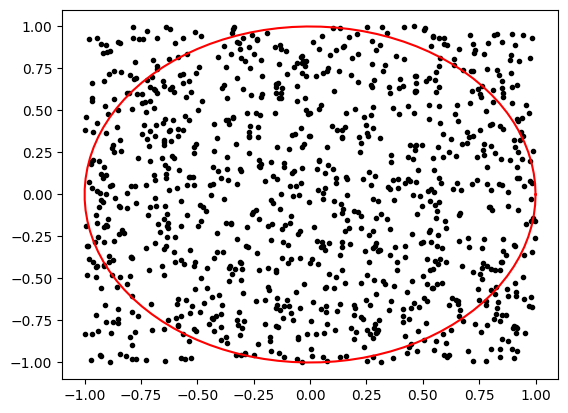
\includegraphics[width=.7\linewidth]{images/Figure1.png}
    \caption{}
    \label{fig:1}
\end{figure}
\begin{figure}[H]
    \centering
    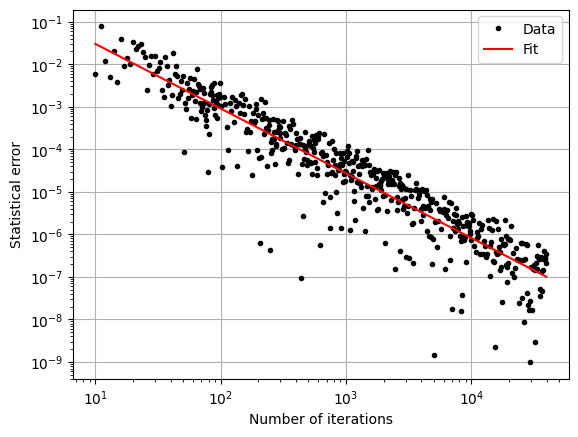
\includegraphics[width=.7\linewidth]{images/Figure1.2.png}
    \caption{log-log plot of the statistical error}
    \label{fig:1.1}
\end{figure}
\begin{figure}[H]
    \centering
    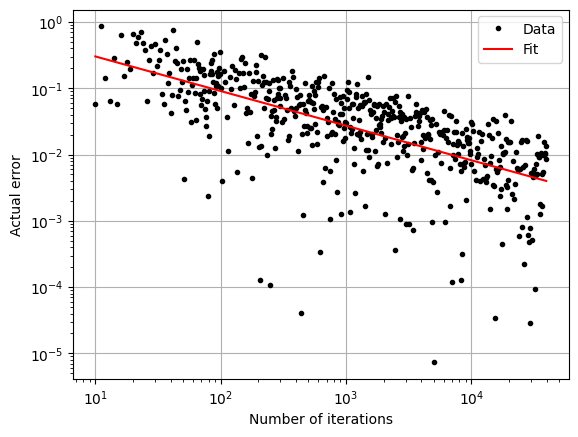
\includegraphics[width=.7\linewidth]{images/Figure1.1.png}
    \caption{log-log plot of the actual error}
    \label{fig:1}
\end{figure}
\clearpage
\section{Volume of a spere in 3D}
Consider a sphere of unit radius, $R=1$, in two dimensions. Generate $N_{iter}$ random numbers using uniform random distribution. Then calculate the probability that point $(x,y,z)$ lies inside of the sphere and use it to approximate the volume of the sphere $V$ and compare it to the exact results: $V_{extact}=\frac43\pi R^3$.\\
As before report the statistical error $\sigma/\sqrt{N_{iter}}$ and compare it with the actual error, then make a log-log plot showing the statistical error and the actual error $|S-S_{exact}|$ as a function of the number of iterations.
\begin{lstlisting}[language=Python]
Niter = 100000
for i in range(Niter):
    a = random.randint(1, 6)
    b = random.randint(1, 6)
    dice_outcome[i] = (a + b) / 2
bin_edges = np.arange(1, 7, 0.5)
counts, _ = np.histogram(dice_outcome, bins=bin_edges)
pdf = counts / Niter
plt.bar(bin_edges[:-1], pdf, width=0.5)
\end{lstlisting}
\begin{figure}[H]
    \centering
    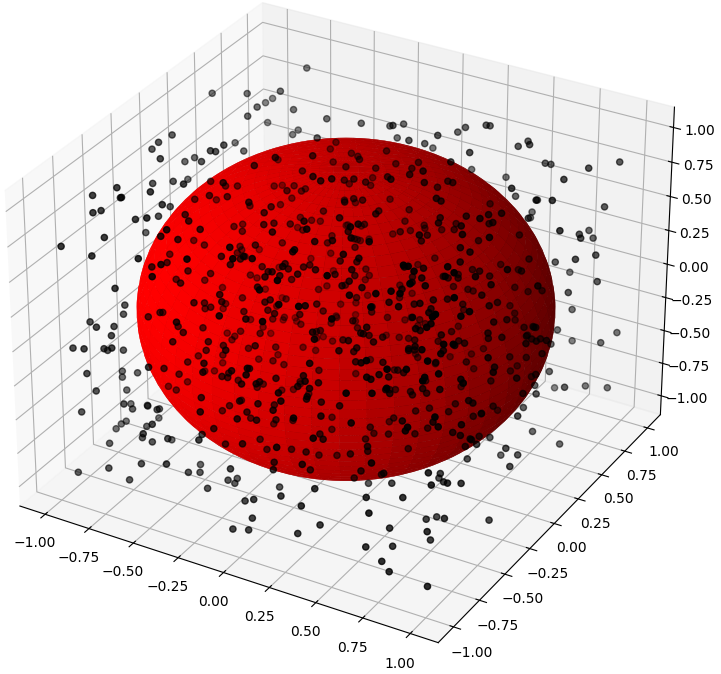
\includegraphics[width=.9\linewidth]{images/Figure2.png}
    \caption{Distribution of the average value of two dice roll}
    \label{fig:2}
\end{figure}
\clearpage
\section{Volume of a sphere in $D$ dimensions}
We now consider the follow random event: throwing a dice $N_{iter}$ times and calculating the average value.
\begin{equation}
    x=\frac{\sum_{i=1}^{N_{iter}}{\text{rand}(6)}}{N_{iter}}
\end{equation}
With that random event $x$ we calculate the probability distribution $p(x)$. As we use large $N$ we can consider the random value $x$ as a continuous variable. And then we normalise the PDF as $\int{p(x)dx}=1$.
With this code we generate calculate the probability distribution:
\begin{lstlisting}[language=Python]
Ndice = 100000
Niter = 10000
def random_event():
    return np.sum([random.randint(1, 6) for _ in range(Niter)])/Niter

random_outcome = [random_event() for _ in range(Ndice)]
hist, bins = np.histogram(random_outcome, bins=50, density=True)
bin_centers = (bins[:-1] + bins[1:]) / 2
plt.plot(bin_centers, hist, label='Computed distribution')

x = np.linspace(min(random_outcome)-0.1, max(random_outcome)+0.1, 1000)
gaussian = norm.pdf(x, loc=3.5, scale=np.std(random_outcome))
plt.plot(x, gaussian, label='Gaussian distribution',color='red', linestyle='--')
\end{lstlisting}
\begin{figure}[H]
    \centering
    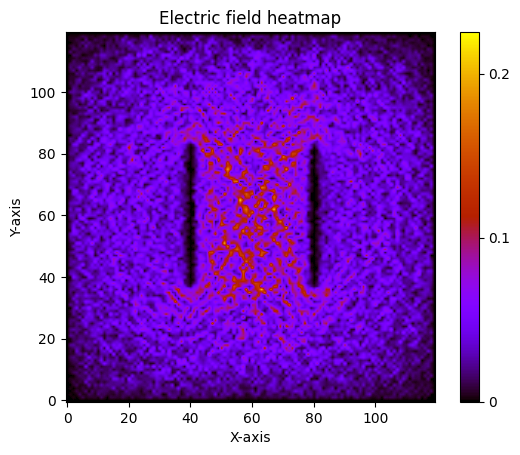
\includegraphics[width=.9\linewidth]{images/Figure3.png}
    \caption{Distribution of the average value of multiple dice roll}
    \label{fig:3}
\end{figure}
As we can see as we use a large number of dice the resulting distribution is pretty similar to the Gaussian distribution expected by the Central Limit Theorem
\clearpage
\section{Error estimation}
We wanna now calculate the average value and estimate the statistical error, associated with such estimation. Assume that single-die throwing is used to estimate the mean value and the variance
\begin{equation}
    \mu=\langle x\rangle\approx\frac{\sum_{i=1}^{N_{iter}}{x_i}}{N_{iter}}
\end{equation}
\begin{equation}
    \sigma^2=\langle x^2\rangle-\langle x \rangle^2\approx\frac{\sum_{i=1}^{N_{iter}}{x_i^2}}{N_{iter}}-\left(\frac{\sum_{i=1}^{N_{iter}}{x_i}}{N_{iter}}\right)^2
\end{equation}
Calculate the mean value by throwing the dice $N_{iter}=10$ and $N_{iter}=100$ times and compare the estimation of the mean value and the variance with the exact values, given by
\begin{equation*}
    \mu=\langle x\rangle=\frac{\sum_{\ell=1}^{6}{\ell}}{6}=3.5\quad \sigma^2=\frac{\sum_{\ell=1}^{6}{\ell^2}}{6}-\left(\frac{\sum_{\ell=1}^{6}{\ell}}{6}\right)^2=\frac{35}{12}\approxeq2.92
\end{equation*}
Using the following code
\begin{lstlisting}[language=Python]
Niter = 10
dice_rolls = np.array([random.randint(1, 6) for _ in range(Niter)])

u = np.sum(dice_rolls)/Niter
var = np.sum(dice_rolls**2)/Niter-np.mean(dice_rolls)**2
\end{lstlisting}
we obatin the results, which are reported in \autoref{tab:1}
\begin{table}[H]
    \centering
    \begin{tabular}{|l|c|c|c|}
        \hline $N_{iter}$  & $\mu$ & $\sigma^2$ &  $\varepsilon $\\\hline\hline
        10 &  &  & \\\hline
        100 &  &  & \\\hline
        1000 &  &  & \\\hline
    \end{tabular}
    \caption{Results of error estimation}
    \label{tab:1}
\end{table}

\end{document}
